\documentclass{article}
\usepackage{graphicx} % Required for inserting images
\usepackage[UTF8]{ctex}

\title{软件课设中期报告\\基于人脸识别的门禁系统设计}
\author{U202111845 王梦婷 \\ U202115980 杨筠松 \\ 指导老师:刘文予}
\date{November 2023}

\begin{document}

\maketitle

\newpage 
\tableofcontents
\newpage

\section{项目背景}
随着近些年来并行化技术的发展,算力瓶颈得到了明显突破,以往只能存在于论文中神经网络,强化学习等数学模型得以迸发惊人的能力,而人脸识别技术这一卷积神经网络(CNN)的核心应用也逐渐广泛应用于每个人的生活中。本项目便是基于人脸识别技术的门禁系统设计,传统的门禁系统需要使用钥匙或者密码进行身份验证,但是这种方式存在一定的安全隐患,例如钥匙丢失或者密码泄漏等问题,而基于人脸识别技术的门禁系统可以通过对用户面部特征的识别来进行身份验证、提高门禁系统的安全性和便捷性。本项目旨在设计并且实现这样一款基于人脸识别技术的门禁系统,为用户提供更加安全、快捷、智能的门禁服务,并且在项目的逐渐实现过程中,增强对AI底层细节的认识,提升对软件系统设计的整体性把握。
\section{需求分析}
为搭建一个基于人脸识别的门禁系统,本项目实现的功能需求如下:

\begin{itemize}
    \item 基本功能:人脸比对
    \begin{itemize}
        \item[-] 新增人脸入库/无效人脸出库
        \item[-] 打卡时间、工作时间、出勤次数记录
        \item[-] 识别失败时或未录入人脸时提供密码验证
        \item[-] 能够现场识别成功提前录入和现场录入的人脸
    \end{itemize}
    \item 附加功能
    \begin{itemize}
        \item[-] 实现人脸跟踪功能,能准确跟踪10s
        \item[-] 实现基于视觉的心率估计功能,误差15\%以内
    \end{itemize}
\end{itemize}

\subsection{数据获取}
人脸是每个人与生俱来的特征,该特征具有唯一性并且不易被复制,从而为身份鉴别提供了必要的前提,我们可以通过opencv中的人脸功能模块,尤其是人脸检测模块、人脸特征值获取模块来实现相应的功能,可以得到如下的数据流程图:

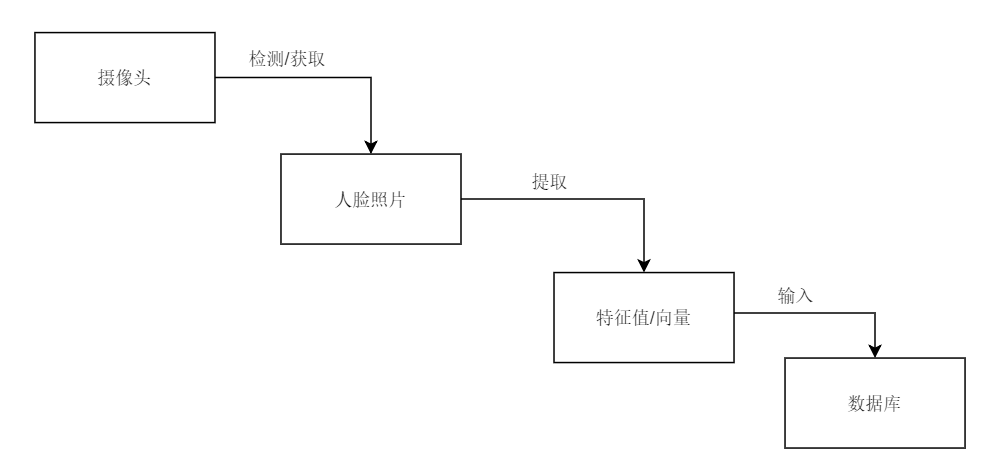
\includegraphics[scale=0.3]{imgs/数据获取.png}

其中可以清楚知道数据将从摄像头获取并且最终合并到数据库中。
\subsection{数据管理}
考虑到数据的来源可能是用户自己照片的上传也可以是调用摄像头的拍摄得到的一帧图像,为保证后续有更多的灵活性,这里采用策略模式(Strategy Pattern)来保证后续方法的可扩展性。而在数据库部分,考虑到数据量较小并且有很大的可扩展空间,初期仅考虑使用文件来作为可持久化数据保存的方式,因为数据库的读写是完全隔离于管理系统本身,而单独作为模块对管理系统提供API,这也为后续随着数据规模的增大,使用更加先进且专业的数据库例如mysql, SQLITE留下可能性,同时降低耦合性提高内聚,将会使得系统变得更加易于后期开发。

当管理员登陆系统后,可以对过期的人脸信息进行删除和修改,同时可以添加新入的人脸以上传图片的方式完成,具体流程如下图所示:

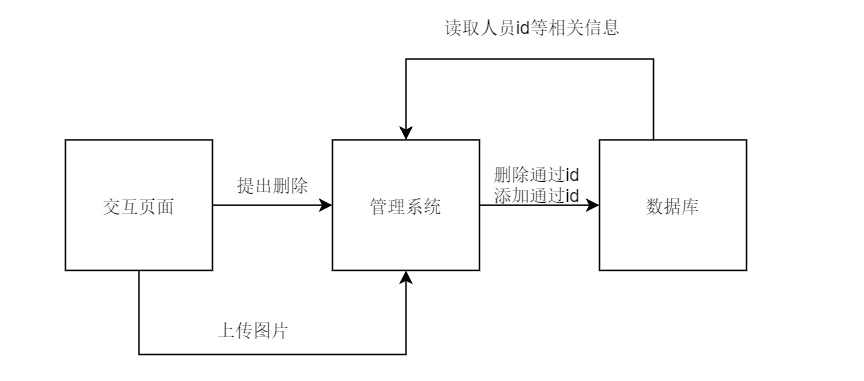
\includegraphics[scale=0.4]{imgs/数据管理.png}

\section{实施方案论证}
\subsection{人脸识别原理剖析}

人脸识别中的核心算法是 PCA 和 SVM,简要介绍如下:
主成分分析(PCA)是一种具有许多实际应用的通用统计方法。当在人脸识别过程中使用时,PCA 旨在减少源数据的大小,同时保留最相关的信息。具体步骤如下:

\begin{enumerate}
    \item 数据预处理:首先,收集一组训练图像,这些图像包含不同人的人脸。然后,对每张图像进行预处理,包括灰度化、对齐和裁剪等操作,以确保图像具有一致的尺寸和方向。
    \item 特征提取:对于每张预处理后的图像,将其转换为一个特征向量。这里使用PCA算法来提取特征。首先,将所有训练图像按照像素展开成一个矩阵,每一列代表一个图像样本。然后,计算这些图像样本的协方差矩阵。接下来,通过对协方差矩阵进行特征值分解,得到特征向量和对应的特征值。这些特征向量称为“特征脸”,它们代表了训练集中的不同人脸。
    \item 降维:根据特征值的大小,选择最重要的特征向量作为主要成分。这些主要成分对应于最大的特征值,它们包含了最多的信息。通过保留较少的主要成分,可以实现对源数据的降维,并减少计算复杂度。
    \item 训练和识别:对于每个人脸图像,计算其在主要成分上的投影。这可以通过将人脸图像与特征脸进行内积运算来实现。将投影结果与训练集中的其他图像进行比较,找到与之最相似的人脸。这可以使用欧氏距离或其他相似度度量来衡量。
\end{enumerate}

经过PCA处理后的图像将会保留主要信息可用于对比,为后续可能的处理提供了便利,而支持向量机(SVM)是一种常用的分类算法,用于将人脸区分成"人脸"和"非人脸"两个类别,这在人脸识别检测中有着举足轻重的影响,具体的步骤如下:

\begin{enumerate}
    \item 数据准备:首先,需要准备一组标记好的训练数据集,其中包括正样本(人脸)和负样本(非人脸)。这些训练数据集应该经过预处理,例如灰度化、对齐和裁剪等操作,以确保图像具有一致的尺寸和方向
    \item 特征提取:对于每张图像,需要提取一组特征向量。这些特征向量应该包含有关每个图像的信息,例如颜色、纹理和形状等。这里可以使用PCA算法来提取特征向量,也可以使用其他特征提取方法。
    \item 训练SVM模型:将训练数据集输入到SVM模型中进行训练。SVM模型通过学习正负样本之间的区别来学习如何将人脸和非人脸区分开来。在训练过程中,SVM模型会寻找一个最优的超平面来分离正负样本。
    \item 测试和识别:在测试和识别阶段,将新的未知图像输入到SVM模型中进行分类。SVM模型会根据已经学习到的正负样本之间的区别来判断该图像是否为人脸。如果该图像被分类为人脸,则可以将其与训练集中的人脸进行比较,并找到与之最相似的人脸。
\end{enumerate}

由此看来PCA和SVM的使用将会造成工作量的骤减,它让原本不可能的计算机视觉变成可能。

\subsection{管理系统类设计}
UML设计图(Version 1.0) 如下所示,随着设计的深入将会后期对UML做出调整

\includegraphics[scale=0.25] {imgs/UML图.png}

\subsection{数据库系统分析}
在最开始的数据库中,我们考虑通过文件类型指针完成对数据的刷入和读取,假设仅仅将id作为主键而不添加任何外键的情况下,读取一条记录需要遍历整个文件即$O(T)$,$T$是整个文件的大小,同样刷入数据或者删除数据也需要$O(T)$的复杂度即需要完成对整个文件刷新,这对本次项目的数据量的需求是足够的。
 
\section{系统架构}
管理系统是整个系统架构的核心,它通过分析从用户端得到的信息在可视化图形界面中给出反馈的同时,还需要对数据库保证数据的安全性和可靠性,如下图所示:

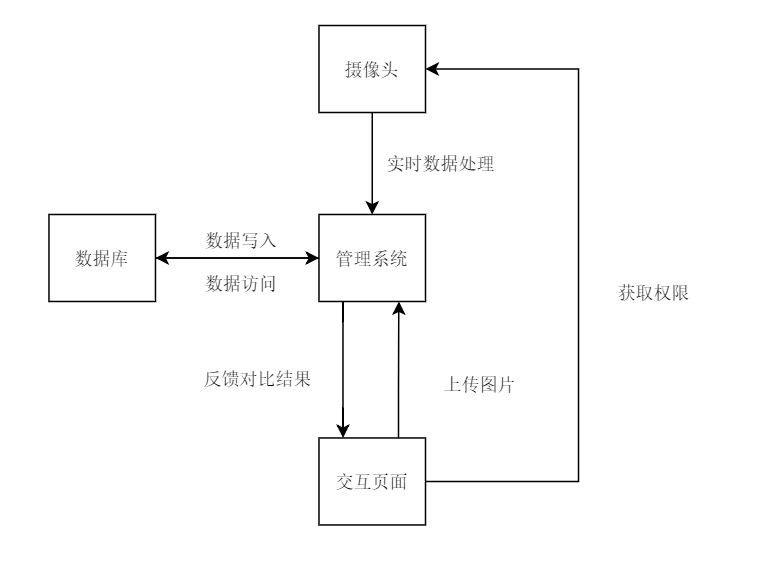
\includegraphics[scale=0.4] {imgs/系统概括.png}

\section{任务分工}

\subsection{人脸识别系统——杨筠松}
\begin{itemize}
    \item 人脸检测+识别模型下载
    \item 人脸图像向量化
    \item 人脸特征比对
    \item 识别逻辑设计
\end{itemize}

\subsection{考勤系统——王梦婷}
\begin{itemize}
    \item 系统UI界面设计
    \item 人脸入库/出库
    \item 考勤信息记录
    \item 多次识别失败+密码考勤
\end{itemize}

\section{进度安排}

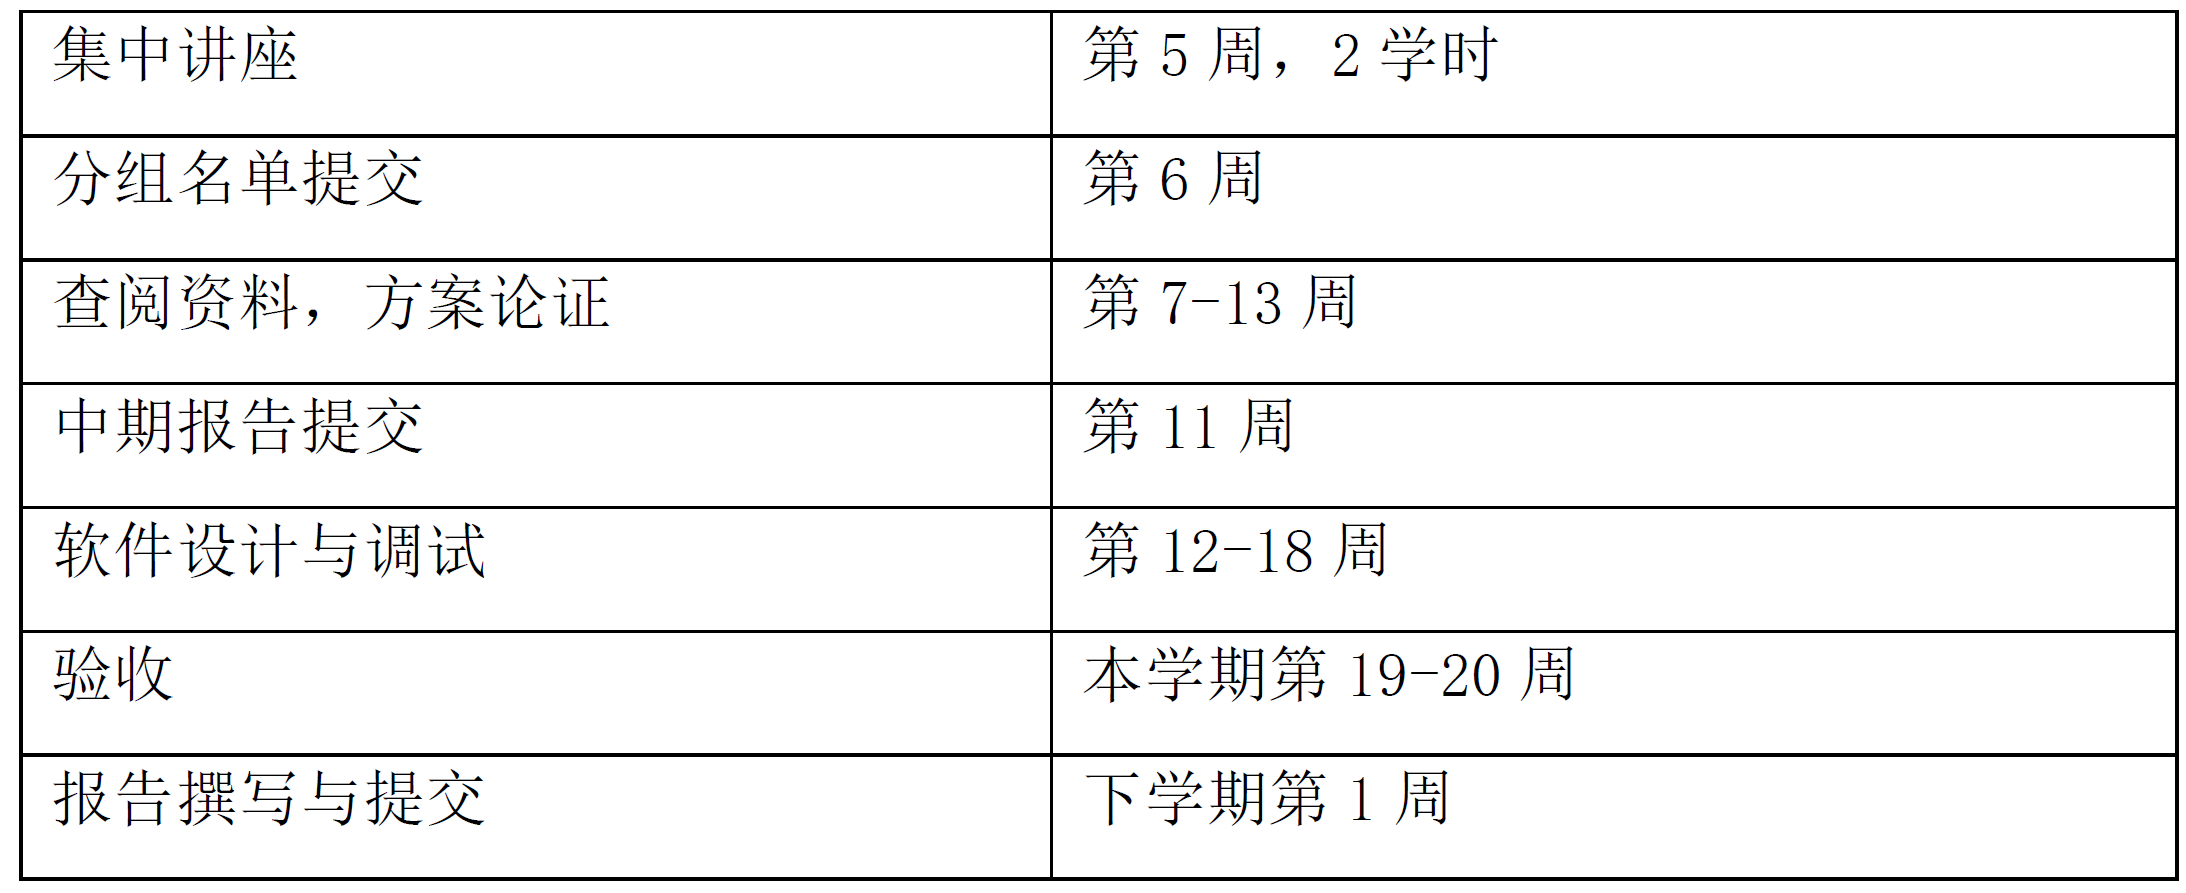
\includegraphics[scale=0.15] {imgs/进度安排.png}

\section{参考资料}
\begin{thebibliography}{00}
\bibitem{b1} https://opencv.org/opencv-face-recognition/
\bibitem{b2} Lavagno, Luciano, Grant Martin, and Bran Selic. UML for Real. Kluwer Academic Publishers, 2003.
\bibitem{b3} Krueger C W. Software reuse[J]. ACM Computing Surveys (CSUR), 1992, 24(2): 131-183.
\end{thebibliography}

\end{document}
